\subsection{VHDL Code}

\sloppy

Die Statemachine der Motorkühlung ist in drei Teile aufgeteilt, dem Zustandsspeicher \glqq STATE\_REGISTER\grqq{}, der Übergangsfunktion \glqq INPUT\_LUT\grqq{} und der Ausgangsfunktion \glqq OUTPUT\_LUT\grqq{}. Das Signal \glqq S\grqq{} ein drei Bit langer Vektor. Die drei Bits repräsentieren die Sensoren der Pumpen. Jeder Sensor gibt ein High- oder Low-Signal aus, je nachdem ob die zugeordnete Pumpe funktionstüchtig ist oder nicht. Da dieses Signal asynchron ist, wird es durch zwei D-Flipflops geführt um mit dem Takt synchronisiert und gepuffert zu werden. Erst nach zwei Taktzyklen empfängt die Übergangsfunktion geänderte Eingangssignale und setzt den nächsten State im Zustandsspeicher. Daraufhin reagiert die Ausgangsfunktion und schaltet je nach zustand die LEDs ein oder aus. Durch diese drei Flipflops wird das Signal um insgesamt drei Taktzyklen verlangsamt.
 
\lstinputlisting[language=VHDL]{code/COOLANT_MONITORING.VHDL}

\subsection{Simulation}

Modelsim .do Datei:

\lstinputlisting[language=tcl]{code/test.do}

\begin{figure}[H]
    \begin{center}
        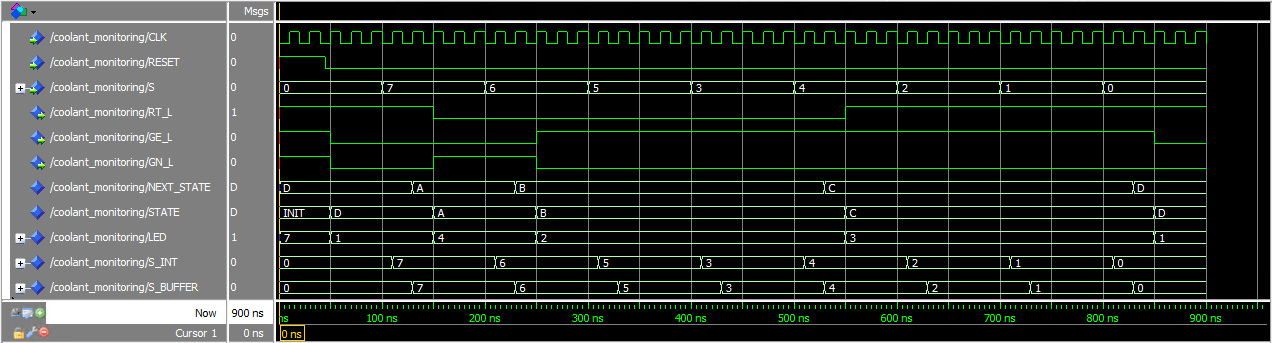
\includegraphics[width=1\textwidth]{img/dip3_sim.png}
        \caption{Simulation}
        \label{fig:A1_sim}
    \end{center}
\end{figure}

\subsection{Auswertung}
Die Startbedingung wird durch den Reset-Eingang erfüllt, beim Start des Automat ist der Resetpin auf eins und setzt den Zustand $Q_0$ auf \glqq INIT\grqq{} um einen definierten Zustand zu erhalten. In diesem Zustand leuchten die Lampen alle auf. Nach drei Taktzyklen sind die Eingangsinformation am Ausgang, also den Lampen, sichtbar. Da alle Pumpen am Anfang auf Low sind, ist der Automat in Zustand D, es Leuchtet die rote Lampe. Nach 6 Taktzyklen wird simuliert, dass alle Pumpen korrekt laufen, also der Eingang drei High-Bits empfängt. Die Schaltung reagiert darauf durch wechseln in den Zustand A, nur die grüne Lampe leuchtet, da alle Pumpen laufen. Im folgenden wird mit einem Abstand von 6 Taktzyklen simuliert, das jede Pumpe nacheinander ausfällt. An den Signalen der Flipflops ist gut die Verzögerung die jedes Flipflop hinzufügt zu erkennen: FF $S_{INT}$, FF $S_{BUFFER}$ und FF State.

